\documentclass[
	fontsize=10pt, % Base font size
	twoside=false, % Use different layouts for even and odd pages (in particular, if twoside=true, the margin column will be always on the outside)
	%open=any, % If twoside=true, uncomment this to force new chapters to start on any page, not only on right (odd) pages
	%chapterprefix=true, % Uncomment to use the word "Chapter" before chapter numbers everywhere they appear
	%chapterentrydots=true, % Uncomment to output dots from the chapter name to the page number in the table of contents
	numbers=noenddot, % Comment to output dots after chapter numbers; the most common values for this option are: enddot, noenddot and auto (see the KOMAScript documentation for an in-depth explanation)
	%draft=true, % If uncommented, rulers will be added in the header and footer
	%overfullrule=true, % If uncommented, overly long lines will be marked by a black box; useful for correcting spacing problems
]{kaohandt}

% Choose the language
\usepackage[english]{babel} % Load characters and hyphenation
\usepackage[english=british]{csquotes}	% English quotes

% Load the bibliography package
\usepackage{kaobiblio}
\addbibresource{main.bib} % Bibliography file

% Load mathematical packages for theorems and related environments
\usepackage{kaotheorems}

% Load the package for hyperreferences
\usepackage{kaorefs}

% Set the paths where to look for images
\usepackage{subcaption}
\graphicspath{{examples/report/img/}{img/}}

\begin{document}

\title{Operation T-REx}
\author[FM]{Federico Marotta}
\date{December 2019}
\maketitle

\chapter*{Introduction}
\addcontentsline{toc}{chapter}{Introduction} % Add the intro to the table of contents as a chapter

Artificial Intelligence (AI) is not magic. It's here, and it's changing the world. Deep learning is one of the most exciting and popular fields of AI, but it's not the same as the good old-fashioned rules-based AI of the past. Deep learning involves training models by repeatedly showing them large datasets and allowing the models to infer the rules between input and output data.

Deep learning models are trained on data, almost like humans. However, the quality of the data is critical to the functioning of the model. For stable and well-understood environments like chess, chemistry or Newtonian physics, we can collect and generate data and deep learning can do a tremendous amount of useful work for us. In less stable environments where the rules of the day sometimes do not reflect the rules of the past, deep learning can be less helpful and even cause real harm when naively deployed. 

I'll discuss dozens of models in detail but consider any data collected that involves complex social interactions. Start with family interactions, then romantic ones and then consider that topics like advertising, trading stocks, credit scoring and even hate speech and threat detection all might have a dynamic social component to them. Models predictive power will suffer if the past does not look like the future. This is a problem for deep learning models that are trained on old data.

Also consider that as a creator of deep learning models, I can use a model to editorialize. I can train a model on data that fits my worldview instead of data that fits the world as it is. As a user or investor, how would you stop me? My stock trading model would be the first one to get me in trouble. If it was regularly monitored and managed, my model could do about as much harm as a troublesome employee could. 

But what about my model that is used to provide online dating advice, credit scores, or acceptance to students to elite universities? It might take a few years before my editorializing was found out, depending on how well it was managed and how egregious my model's outputs are.

Some of these problems are small potatoes, who cares if online dating sites don't do good science to suggest matches? What about full-self driving though? The realization of autonomous cars we're told is perpetually years away, but is it really possible with our current roads, laws and infrastructure? What happens if a model stops being updated, and it becomes the height of fashion for kids to wear shirts with street-signs on them? Do all of the cars stop working? Also, we're calling this autopilot, but don't pilots in planes need to file flight plans, speak to other planes and take instructions from a tower? Do our cars need to do that too? 

If you understand the type of AI that is being used (rules-based or deep learning), the data it was trained on, and monitor the AI in production you are on the road to success. But, what if I told you I could use the outputs from the model you just spent a billion dollars building and very easily create a new model that performs almost as well, and spend almost nothing building it. Furthermore, if you took me to court I could show my work and prove that I made the model myself. Would this change the way you invest in artificial intelligence? Would it change the way you develop and share your models?

Back to self-driving cars, Here is how that could pan out. Imagine Honda comes from behind and creates the worlds greatest fully self-driving car and it cost them only \$1 billion to make. Now imagine I buy a couple of those Hondas, maybe 100 of them for \$30,000 each, then pay 100 drivers \$100,000 per year to drive them, and equip each honda with \$70,000 of my own computers and sensors. At the end of this endeavour I could theoretically create a decent machine learning model using the "Honda's" data for 20\% of their investment. There are of course other costs I would incur, but if you come along with me and assume that the data is the most important component of the model, then I have all of the data I need on the cheap.

I'll disucss this in detail in chapter 5, but for now let me tell you I'm skeptical of full self-driving without a lot of infrastructure changes, but I'm not skeptical of the ability to create a model that can drive a car. I'm skeptical of the ability to create a model that can drive a car in a way that is safe, reliable and that will hold up in court.   

The cost of innovating is well known, and this is why patent protection exists. But deep learning models are trained on data that is free or easy to copy and in a way that produces slightly different and seemingly random inner-workings on each training run, if this is the case then I don't see many defensible positions for innovators in machine learning. Let's consider another hypothetical from pharmacology, imagine Pfizer invented the cancer curing pill, then I put that pill in a machine that came up with a significantly different formulation that achieved the same results, and when you gave it to the expert witness chemists they would have to say "the chemistry of these two pills is fundamentally different, but they both cure cancer", which would make it very hard to defend the original cancer pill's patent in court.

Because of the way they are trained, deep learning models introduce real mathematical chaos wherever they are deployed. This leads me to a few conclusions that I'll give you here in the introduction, but explain in detail in the meat of this book: 

\begin{enumerate}
\item Deep learning models can make statistically informed decisions based on the data they were previously shown, but because of their size they can produce seemingly random results. Poor data collection (or editorializing) leads to poor results. Anything using deep learning models cannot be used by itself to make critical decisions. Said differently, there must be supervision and outside control wherever deep learning is involved.
\item Any decision involving deep learning models is functionally unexplainable, and therefore likely to get someone in trouble in court. Any domain where deep learning is used to make a decision and then asked to explain in detail how that decision was made should be greeted with a shrug from the witness stand.
\item Deep learning intellectual property is indefensible, it is built in a way that is both easily copyable, and impossible to verify that it was actually copied.
\end{enumerate}

Deep learning introduces challenges for some, but opportunities for others. I am a member of the \href{https://www.fsf.org/}{Free Software Foundation}, and from my perspective deep learning models are one type of software that might inherently support the foundation's purpose. The purpose of the foundation is to promote the universal freedom to distribute and modify computer software without restriction. If deep learning models are simultaneously powerful and free, they become rocket fuel for innovation. 

This is the silver lining to the "myths" that I'd like to discuss in this book. Deep learning is messy, data science is hard, but as a tool deep learning is absolutely mindblowing. I can rank order my emails by their sarcasm, create avatars of my friends in the style of Disney characters, have ChatGPT summarize the DaVinci Code for my book report, and have my deep learning model suggest possible life saving drugs for me. The world is fantastic and will get better thanks to this tool, but like any tool we should use it safely and appropriately.  

Consider utilizing deep learning as an "employee" for any non-critical tasks that you don't wish to perform yourself. I personally fired my virtual assistant from Brickwork India (\$200/month) and hired ChatGPT (\$20 per month). By managing it, you can put yourself in an excellent position. In my opinion, the world won't end up in a dystopian \href{https://en.wikipedia.org/wiki/The_Terminator}{\textit{Terminator}}-esque state, nor will work disappear in a utopian \href{https://en.wikipedia.org/wiki/Fully_Automated_Luxury_Communism}{\textit{Fully-Automated Luxury Communism}} scenario. Instead, we'll find ourselves somewhere in the middle, and it'll likely be more gratifying. Work will transform, we will supervise and manage our new technological workers, and they'll be cheap! This new management job won't require us to give up our agency but to act as masters of a new realm where our attention and thought are required, and where vital decisions are still made by us.

\section{Data}
\labsec{data}

The Genotype-Tissue Expression (GTEx) project \sidecite{Lonsdale2013a} 
aims to characterise gene expression and regulation for 54 human healthy 
tissues across nearly 1000 people. While the results of the analyses are 
open-access, in order to gain access to the raw data about the DNA and 
the gene expression of the individuals, it is necessary to go through a 
long bureaucratic procedure.

Another source of data was the Ensembl project (release 75), 
\sidecite[-1.55cm]{Zerbino2018} which was used to obtain the coordinates 
of the regulatory regions for each gene. Regulatory regions are 
particular positions around a gene where transcription factors can bind; 
from there, these transcription factors exert a control on gene 
expression.\sidenote{In this project, I considered 141 genes of a 
particular type of blood cells, for 95 individuals. Each gene is 
associated to about 10 regulatory regions on average.} Each 
transcription factor recognises a specific sequence of DNA, therefore it 
is possible to compute the affinity of a factor for a given region. The 
total binding affinity (TBA) \sidecite[-3.85cm]{Molineris2011a} is one 
of the possible affinity measures.\sidenote[][]{The TBA is also 
related to the name of this project, T-REx: indeed, the goal is to 
estimate the TBA-Regulated Expression.}

Gene expression in GTEx was measured with a technique called 
RNA-sequencing, which returns, for each gene and each individual, the 
RPKM, \sidecite[-4.6cm]{Mortazavi2008} which is the number of sequencing 
reads normalised by the length of the gene and by the total number of 
reads.

%\begin{figure}[H]
\begin{figure}[H]
  \begin{subfigure}{\textwidth}
	\centering
	\caption{}
%	\caption{Histogram and normal Q\babelhyphen{nobreak}Q plot of the 
%expression of a randomly selected gene called BID. In the histogram, the 
%brown dashed line indicates the mean, while the dotted lines indicate 
%plus and minus one standard deviation. In the Q\babelhyphen{nobreak}Q 
%plot, each point represents an individual.}
	\labfig{distrexpr}
	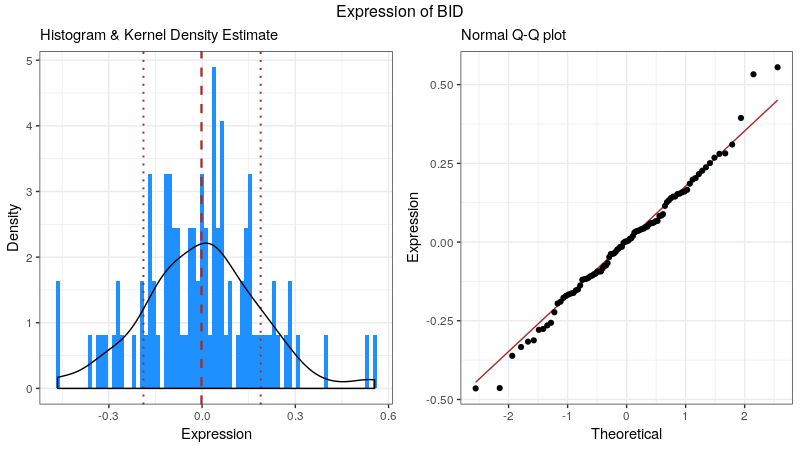
\includegraphics[height=4.8cm,width=.8\textwidth,keepaspectratio=false]{bid_expr}
  \end{subfigure}
%\end{figure}

  \begin{subfigure}{\textwidth}
%\begin{figure}[t]
    \centering
    \caption{}
% 	\caption{Scree plot and biplot of 
% the \textasciitilde800 affinities for the gene BID. In the biplot, each 
% label corresponds to an individual.}
    \labfig{pcatba}
    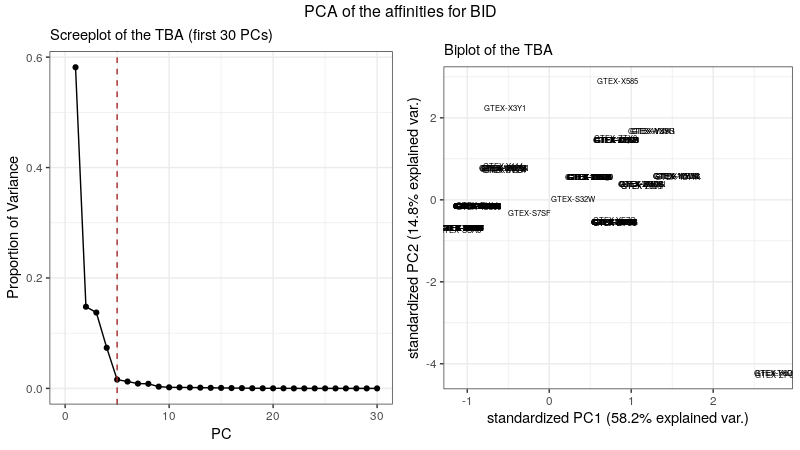
\includegraphics[height=4.8cm,width=.8\textwidth,keepaspectratio=false]{bid_tba}
  \end{subfigure}
% \end{figure}
  \caption{(a): Histogram and normal Q\babelhyphen{nobreak}Q plot of the 
expression of a randomly selected gene called BID. In the histogram, the 
brown dashed line indicates the mean, while the dotted lines indicate 
plus and minus one standard deviation. In the Q\babelhyphen{nobreak}Q 
plot, each point represents an individual. (b): Scree plot and biplot of 
the \textasciitilde800 affinities for the gene BID. In the biplot, each 
label corresponds to an individual.}
  \labfig{expl}
\end{figure}

The expression was preprocessed as recommended by the Stephen's 
Lab.\sidenote[][*7]{\url{http://stephenslab.github.io/gtex-eqtls/analysis/20170515\_RNASeq\_Analysis.html}} 
In summary, I applied a quantile normalisation to make sure that the 
distribution of our response variable was normal, and then I obtained 
the residuals of a linear model 
$Y~\sim~SEX+PEER\_FA+POPULATION+PLATFORM$, so as to disregard the 
effects of these covariates on the expression. The final result can be 
seen in \reffig{distrexpr}.

The genotypes were also obtained with a sequencing technique and were 
provided in VCF format. \sidecite[-3.2cm]{Danecek2011} I 
used a software called 
\nohyphens{VCF\textunderscore\nobreak\hspace{0pt}rider}\sidenote[][*3]{\url{https://github.com/vodkatad/vcf\_rider}} 
to compute the total binding affinity of each transcription factor for 
each regulatory region associated to a gene (the total number of 
transcription factors is about 800). \reffig{pcatba} reports the PCA of 
the TBA for the gene BID.

\section{Results}
\labsec{results}

\subsection{Nested Cross-Validation Package}

All the similar published works use a 5-fold cross-validation to 
evaluate their models. However, since there are also some parameters to 
tune, they rely on a (computationally expensive) netsed cross-validation 
in order not to overestimate the predictive power. Since I needed to run 
several different models for each of the 140 genes, each with its own 
parameters, I decided to write an R 
package\sidenote[][-2.3cm]{\url{https://github.com/fmarotta/cvtools}} to 
perform the nested cross-validation with a heuristic algorithm that does 
not try all the possible values for the parameters, but rather, 
independently for each parameter, it starts at one value and explores 
the adjacent ones; then, it moves in the direction where the error 
decreases
(\reffig{cv}).

\begin{marginfigure}[-3.4cm]
  \centering
  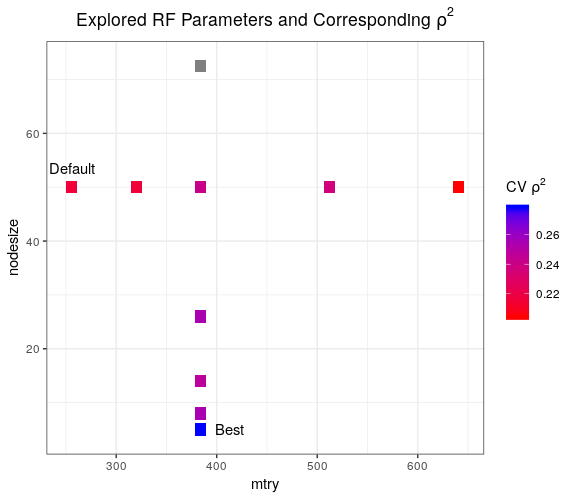
\includegraphics{cv}
  \caption{First, the mtry is tuned while the nodesize is kept fixed; 
the algorithm started at the default value of 256, then it moved up in 
the range as long as the error decreased, and finally it came back to 
explore the values in between. Next, the nodesize was tuned in a similar 
fashion.}
  \labfig{cv}
\end{marginfigure}

This package requires the user to write a function which takes 
predefined arguments and returns a predefined output, but except for 
that, it can be used with any regression model. I evaluated the 
performances of ridge, BART, random forest, and PCR. 
\sidecite[-12.9cm]{James2013a,Hastie2009}

\subsection{Model Performance}

The measure of performance is not the MSE nor the $R^2$, but rather the 
square of the correlation between true and predicted expression 
($\rho^2$); indeed, we do not want to penalise errors on single 
individuals, but we are interested in the general trend of expression. I 
decided to compare my results with those of TIGAR, \cite{Nagpal2019} 
which is currently most recent paper on this topic.

\begin{table}[b]
  \caption{Mean $\rho^2$ across 141 genes. The t-test was always 
performed with respect to TIGAR.}
  \labtab{comp}
  \begin{tabular}{lcc}
  \textbf{Model} & \textbf{Mean} \boldmath$\rho^2$ & \textbf{t-test pval} \\
  \midrule
  TIGAR & 0.067 & NA\\
  Ridge & 0.076 & 0.025\\
  BART & 0.074 & 0.121\\
  Ranger & 0.069 & 0.398\\
  PCR & 0.064 & 0.737\\
  \end{tabular}
\end{table}

Even if it captures only the linear relationships, ridge gave the best 
predictive performance (\reffig{rho2distr}), probably because in this 
context where $p >> n$, it is a good compromise between bias, variance 
and overfitting. According to a t-test, the $\rho^2$ achieved by ridge 
with the TBA values are even higher than those obtained by TIGAR 
(\reftab{comp}).

\begin{marginfigure}[-2cm]
  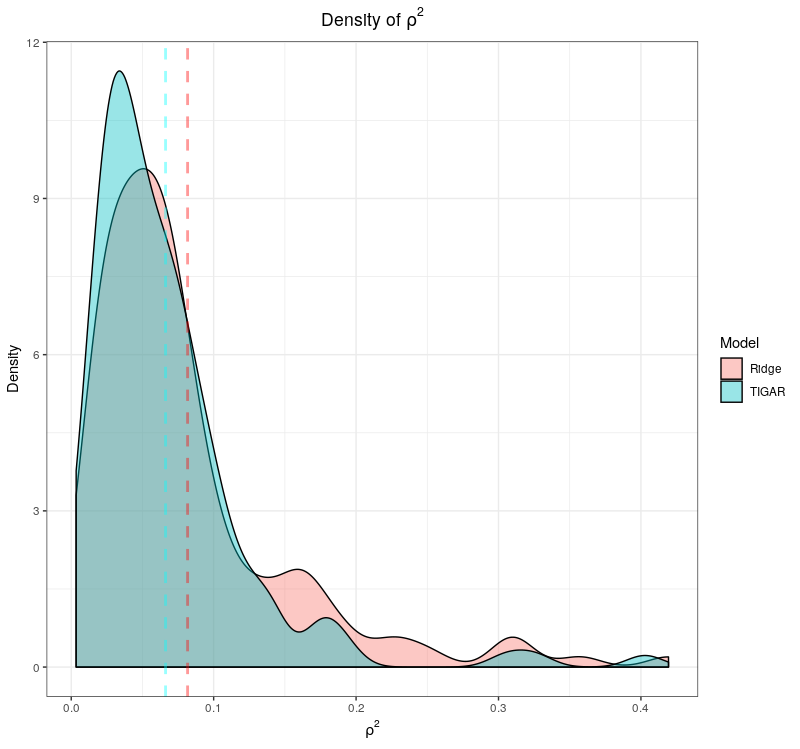
\includegraphics{rho2distr}
  \caption{Density plot of the $\rho^2$ achieved by T-REx (Ridge) and 
TIGAR. The dotted lines denotes the means of the 
distributions.}
  \labfig{rho2distr}
\end{marginfigure}

The performance of BART was not so different, despite the method being 
completely different. However, an important advantage of BART with 
respect to ridge is its ability to provide importance measures, allowing 
us to find which transcription factors are important for each gene. 
Additionally, BART captures the interactions between transcription 
factors.

The other methods, random forest and principal component regression, 
were much less powerful.

\subsection{Considering the Expression of the Transcription Factor}

As high as its affinity for the DNA may be, if the transcription factor 
is present only in tiny amounts it will not bind many regulatory 
regions. For this reason, we tried to enhance our predictors with 
information from the expression of the transcription factors.

\marginnote{%
The Hill equation models the rate of expression of a gene:
\begin{equation*}
  \theta = w \frac{L^n}{K^n + L^n} \approx w \left(\frac{L}{K}\right)^n.
\end{equation*}
Here, $L$ is the amount of transcription factor, $K$ is the dissociation 
constant (the inverse of the affinity), and $w$ is a constant. It is 
reasonable to suppose that if many transcription factors regulate a 
gene, the rate will be given by the following product, where we denoted 
$A = 1 / K$:
\begin{equation*}
  \theta = w_1 \left( L_1 A_1 \right)^{n_1} \cdots w_p \left( L_p A_p \right)^{n_p}.
\end{equation*}
Now, if we compute the log of the rate, we get a linear combination 
which in principle is a deterministic function, but in practice we can 
use this linear combination as the right-hand side of a model formula 
and let ridge estimate the coefficients:
\begin{align*}
  Y \sim \beta_0 &+ \beta_1 \left(\log L_1 + \log A_1\right) \\
                 &+ \cdots \\
                 &+ \beta_p \left(\log L_p + \log A_p\right).
\end{align*}
}

In the dataset, we have expression values for some 40.000 genes; of 
these, about 800 are transcriptional factors. In practice we removed 
those rows from the dataset, and summed the TBA and the expression of 
corresponding transcription factors. The new predictors gave a 
considerable improvement in the performance, and, perhaps surprisingly,
ridge outclassed BART. In the adjacent margin note I describe the 
working hypothesis more in detail.

\begin{table}[H]
  \begin{tabular}{lr}
  \textbf{Model} & \textbf{Mean} \boldmath$\rho^2$ \\
  \midrule
  Ridge & 0.393\\
  BART & 0.268\\
  \end{tabular}
\end{table}


\section{Discussion}
\labsec{discussion}

Instead of finding a better model, in this project I tried to find 
better predictors. Using the affinities instead of the genotypes has 
several advantages:

\begin{itemize}
  \item The model is more interpretable;
  \item The number of predictors decreases;
  \item The predictive power is higher;
\end{itemize}

Upon doing some biochemical considerations, it is possible to find even 
better predictors, although they violate the constraint of using only 
the DNA sequence to predict gene expression.

There are many ways to continue this work. One would be to construct an 
ensemble model that chooses, for each gene, the model that achieved the 
best prediction on a training set.

Another possibility is that of exploiting further the interpretability 
of this model, and use the trees produced by BART to make inferences 
about the regulatory network among genes.

Finally, one of the biggest limitations of these kind of models is that 
they consider each gene as independent of all the others. One possible 
way to use the information hidden among other genes is what I call the 
\enquote{bagging of the genes,} where the prediction for a new gene is 
given by the average of the prediction of a number of other models 
trained on different genes.

If we were able to accurately predict gene expression, the benefit would 
be twofold: first, it would be possible to predict which individuals are 
at risk of developing a disease, and consequently to prevent it; 
secondly, the biological mechanisms through which the illnesses arise 
would be elucidated, potentially leading to the discovery of new 
therapeutic targets. In conclusion, I hope that this project will give a 
contribution, albeit very small, in understanding the relationships 
between genome, expression and diseases.


\defbibnote{bibnote}{Here are the references in citation order.\par\bigskip} % Prepend this text to the bibliography
\renewcommand*{\bibfont}{\small}
\printbibliography[title=Bibliography]% , prenote=bibnote]

\end{document}
